\documentclass[compress]{beamer}
\usepackage[utf8]{inputenc}
\usepackage[T1]{fontenc}
\usetheme{Singapore}
\usecolortheme{default}
\usepackage{graphicx}

\begin{document}
\title{Verschlüsselung mit GPG}  
\author{Sokü \& friends}
\date{} 

\frame{\titlepage} 

\frame{
  \frametitle{Struktur}
  \tableofcontents
} 

\section{Motivation}
\label{sec:motivation}

\begin{frame}
  \frametitle{Warum das alles eigentlich?}

  \begin{itemize}[<+(1)->]
  \item Emails können sehr leicht mitgelesen werden.
  \item Nur wer ein bisschen die Technik versteht, kann sich bewusst
    verhalten.
  \end{itemize}
\end{frame}

\section{Theorie}
\label{sec:theorie}
\begin{frame}
    \frametitle{\insertsection}
    \begin{description}
        \item[Verschlüsselung] Ich will nicht, dass alle wissen, was ich schreibe.
        \item[Authentifikation] Ich will mit der richtigen Person sprechen.
    \end{description}
\end{frame}

\subsection{Symmetrische und Asymmetrische Verschlüsselung}
\begin{frame}
  \frametitle{\insertsubsection}
  \begin{overprint}
    \onslide<1-4>
    \begin{description}
    \item[Symmetrische Verschlüsselung:] \alert{Ein} Schlüssel
      zum Verschlüsseln und wieder Entschlüsseln.
      
      \onslide<4>{Der Schlüssel muss sicher von der Senderin zum
        Empfänger gebracht werden. (alte Agentenfilme: Aktenkoffer mit
        Selbstzerstörung und so)}
    \end{description}
    \onslide<5-7>
    \begin{description}
    \item[Asymmetrische Verschlüsselung:] Zwei Schlüssel: Ein
      \alert{öffentlicher} nur zum Verschlüsseln (darf auch den Bösen
      bekannt sein) und ein \alert{privater} zum Entschlüsseln
      (geheim, muss aber nicht mehr quer durch die Stadt getragen
      werden).
    \end{description}
  \end{overprint}
  \vspace{1em}
  \begin{overlayarea}{\columnwidth}{8em}
    \includegraphics<2>[width=\columnwidth]{bilder/symmetric_schluessel.png}
    \includegraphics<3>[width=\columnwidth]{bilder/symmetric_text.png}
    \only<4>{
      \begin{center}
        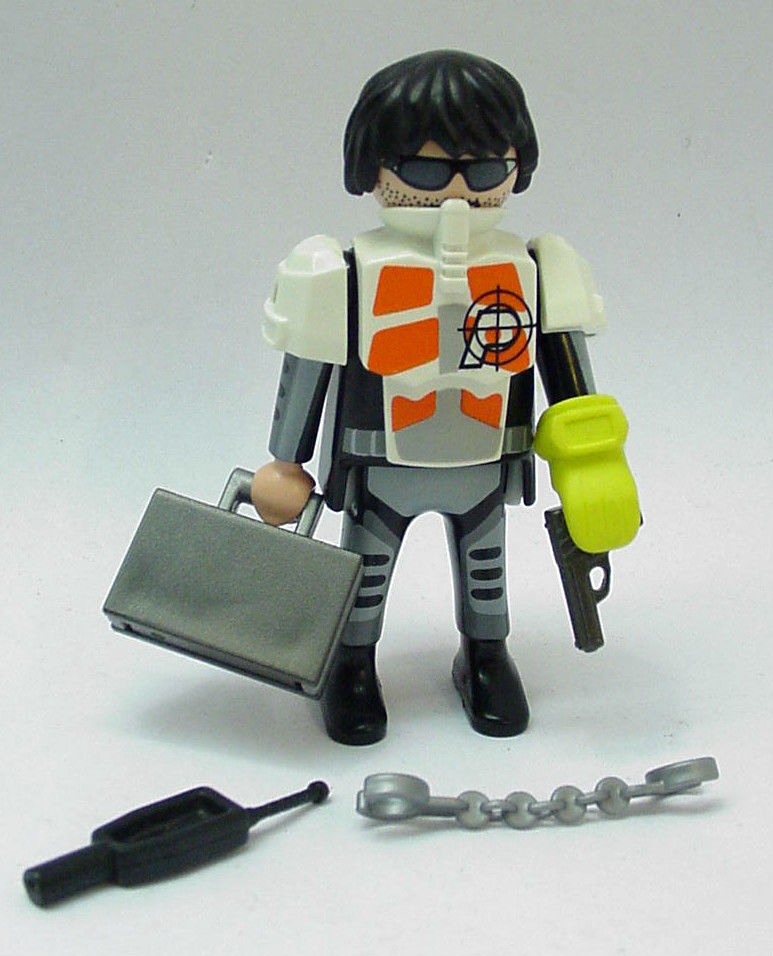
\includegraphics[height=9em]{bilder/agent_koffer.jpg}
      \end{center}
    }
    \includegraphics<6>[width=\columnwidth]{%
      bilder/public_key_verfahren_schluessel.png}
    \includegraphics<7>[width=\columnwidth]{%
      bilder/public_key_verfahren_text.png}
  \end{overlayarea}

\end{frame}

\begin{frame}
  \frametitle{\insertsubsection}
  \begin{description}
  \item [Wie geht das?] Mathe!  Zahlen multiplizieren geht leicht,
    Zahlen wieder aufteilen nicht.
  \end{description}
  \begin{center}
    
\includegraphics[width=0.9\columnwidth]{bilder/math1.png}\\
    
\includegraphics[width=0.9\columnwidth]{bilder/math2.png}
  \end{center}
\end{frame}

\subsection{Primzahlen rechnen}
\begin{frame}
  \frametitle{\insertsubsection}
  \begin{description}
  \item[Taschenrechner dabei?] \mbox{}\\
    \begin{itemize}
    \item<1-> 7 x 11 = ?
    \item<2-> 65 = \only<2>{? x ?}\onslide<3->{5 x 13}
    \item<4-> 11251 x 2953 = \only<4>{?}\onslide<5->{33224203}
    \item<6-> 12883649 = \only<6>{? x ?}\onslide<7->{2957 x 4357}
    \end{itemize}
  \item[Verschlüsselung?]<8-> Das Produkt aus den zwei Primzahlen ist
    in etwa der öffentliche Schlüssel (auch die Geheimdienste können
    die Zahl nicht wieder aufspalten), die zwei kleinen Zahlen sind
    der private Schlüssel und müssen geheim bleiben.
  \end{description}
\end{frame}

\section{Theoretische Praxis}
\label{sec-1-1-4}

\begin{frame}
    \frametitle{Pretty Good Privacy}
    \onslide<2>
    Eine Methode asymmetrische Verschlüsselung umzusetzen ist
    \alert{P}retty \alert{G}ood \alert{P}rivacy, kurz PGP.
    \begin{itemize}
        \item de-facto Standard für Email-Verschlüsselung
        \item benutzt Primzahlzerlegung
        \item stellt Signaturen bereit
    \end{itemize}
\end{frame}
\begin{frame}
    \frametitle{Schlüsselerstellung}
    \begin{description}
        \item[Theorie:] Generiere zufällige große Primzahlen
        \item[Praxis:] Maus bewegen
    \end{description}
\end{frame}
\begin{frame}
    \frametitle{Schlüsselaustausch}
    \begin{description}
        \item[Persönlich (USB-Stick)] sehr umständlich, aber sicher
        \item[Mail:] weniger umständlich, unsicher
        \item[Schlüsselserver:] Das schwarze Brett für PGP-Schlüssel
    \end{description}
    % Schlüsselaustausch und -server
\end{frame}
\begin{frame}
    \frametitle{Authentifikation}
    % Fingerprints und Signaturen
    Wem gehört der PGP-Schlüssel?
    \begin{description}
        \item[Signatur:] unterschreiben von Inhalten mit geheimen Schlüssel
        \item[Fingerprint:] Abbild vom öffentlichem Schlüssel
    \end{description}
    Signierte Mails reichen nicht, die Signatur muss auch stimmen!
    \onslide<2>
    \begin{itemize}
        \item Signieren von öffentlichen Schlüsseln möglich
        \item Überprüfen, ob die Mailadresse und öffentlicher Schlüssel zur Person passen
        \item Danach den Schlüssel signieren und auf Schlüsselserver laden
        \item Keysigning parties
    \end{itemize}
\end{frame}
\begin{frame}
    \frametitle{Widerrufen von Schlüsseln}
    Was tun wen's brennt?
    \begin{itemize}
        \item Passwort vergessen
        \item Private Key verloren
        \item Rechner beschlagnahmt
    \end{itemize}
    Der Schlüssel darf nicht mehr verwendet werden!
    \onslide<2>
    \alert{Widerrufszertifikat} erklärt den Schlüssel für ungültig.

    Weiter: Ablaufdatum für Schlüssel
\end{frame}

\section{Die Praxis in der Theorie}
\label{sec-1-1-5}

\begin{frame}
  \frametitle{\insertsection}
  Programme zum Verschlüsseln:

  \begin{description}
  \item[gpg] \alert{G}nu\alert{P}rivacy\alert{G}uard, ein Programm zum
    Verschlüsseln und Signieren.  Heißt auf Windows \alert{GPG4Win}.
  \item[Enigmail] Ein Plugin für das Thunderbird-Mailprogramm, das gpg
    verwendet, um Mails zu verschlüsseln.
  \item[\ldots] Programme können auf anderen Systemen auch anders
    heißen.
  \end{description}

\end{frame}

\begin{frame}
  \frametitle{\insertsection{} -- Installation GPG4Win}
  \centering
  \only<+>{
    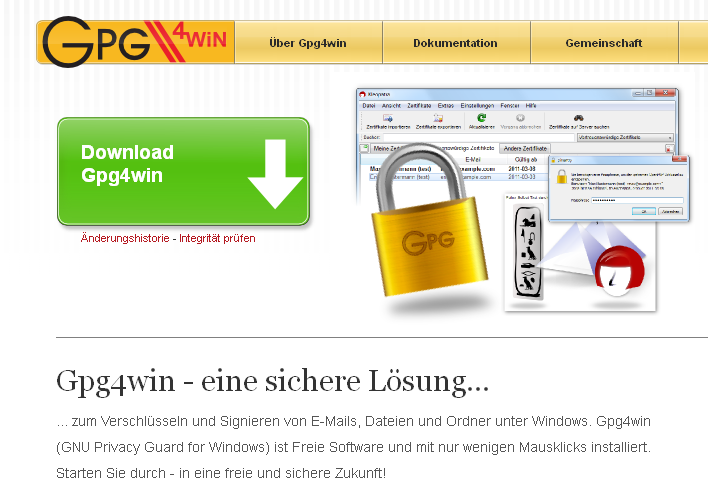
\includegraphics[width=\columnwidth]{bilder/gpg_download}
  }
  \only<+>{
    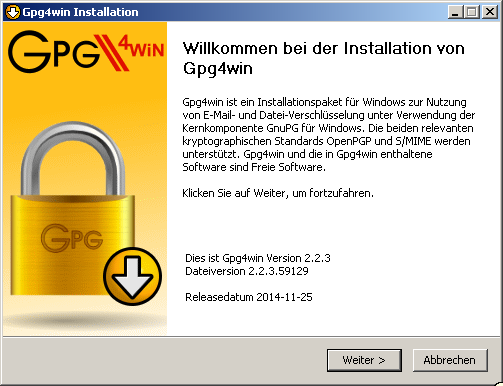
\includegraphics[width=0.7\columnwidth]{bilder/gpg_installation}
  }
\end{frame}

\begin{frame}
  \frametitle{\insertsection{} -- Installation Enigmail}
  \centering
  \only<+>{
    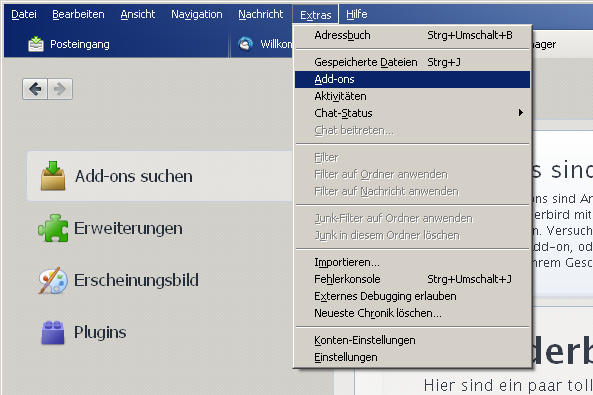
\includegraphics[width=\columnwidth]{bilder/enigmail_addons}
  }
  \only<+>{
    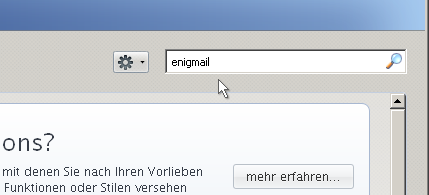
\includegraphics[width=\columnwidth]{bilder/enigmail_suche}
  }
  \only<+>{
    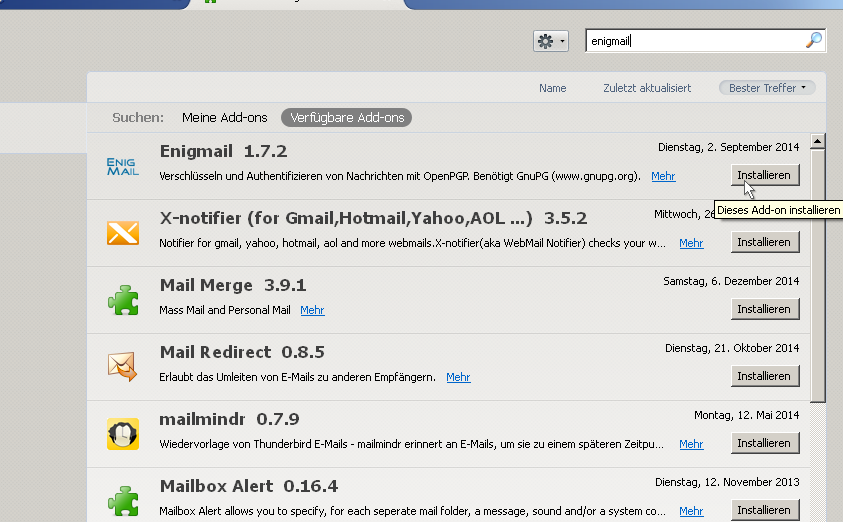
\includegraphics[width=\columnwidth]{bilder/enigmail_gefunden}
  }
  \only<+>{
    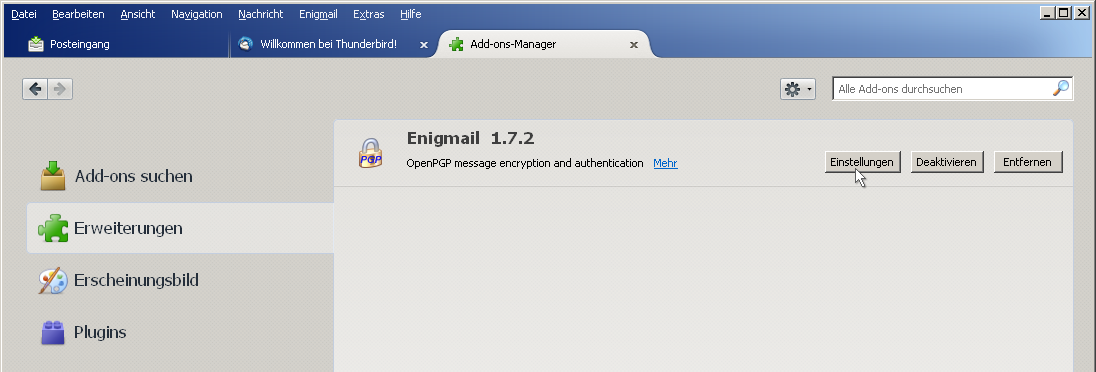
\includegraphics[width=\columnwidth]{bilder/enigmail_einstellungen}
  }
\end{frame}

\begin{frame}
  \frametitle{\insertsection{} -- Schlüsselgenerierung}
  \centering
  \only<+>{
    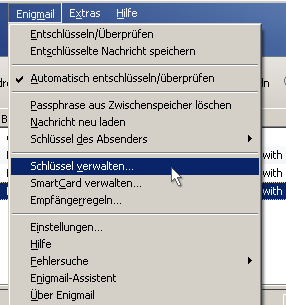
\includegraphics[width=0.5\columnwidth]{bilder/schluessel_verwalten}
  }
  \only<+>{
    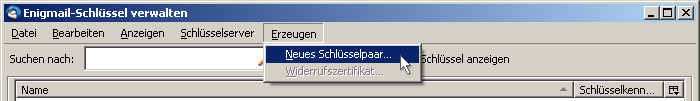
\includegraphics[width=\columnwidth]{bilder/neues_schluesselpaar}
  }
  \only<+>{
    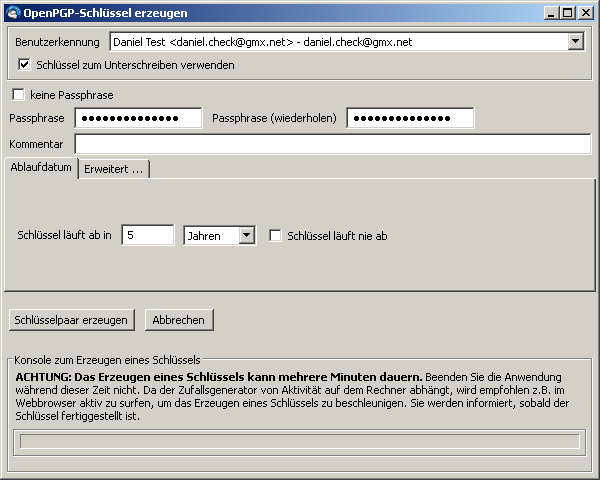
\includegraphics[width=0.8\columnwidth]{bilder/schluessel_erzeugen}
  }
  \only<+>{
    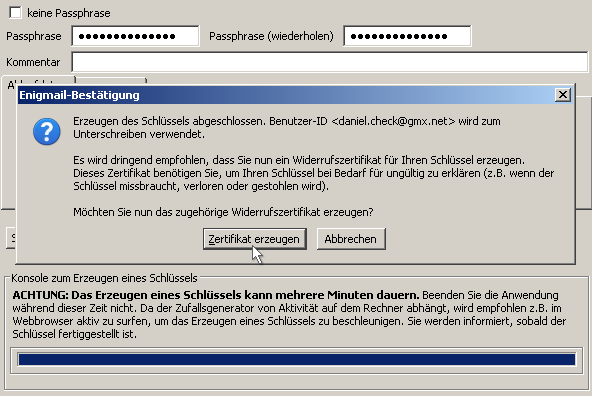
\includegraphics[width=0.8\columnwidth]{bilder/widerruf_erzeugen}
  }
  \only<+>{
    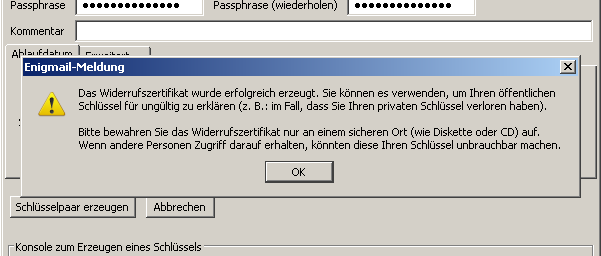
\includegraphics[width=0.8\columnwidth]{bilder/widerruf_erzeugt}
  }
  \only<+>{
    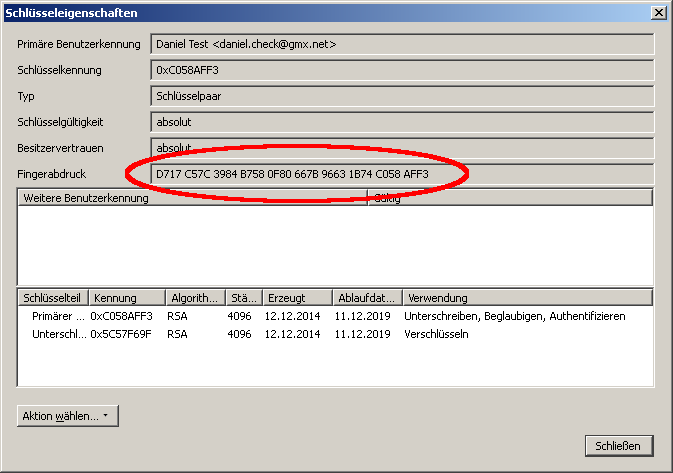
\includegraphics[width=\columnwidth]{bilder/schluessel_eigenschaften}
  }
\end{frame}

\begin{frame}
  \frametitle{\insertsection{} -- Schlüssel hochladen}
  \centering
  \only<+>{
    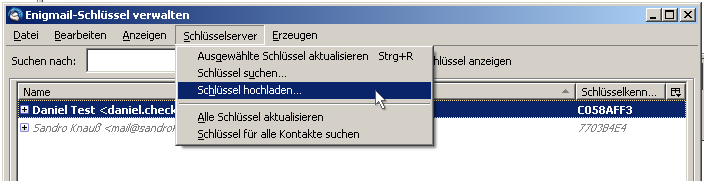
\includegraphics[width=0.95\columnwidth]{bilder/schluessel_hochladen}
  }
  \only<+>{
    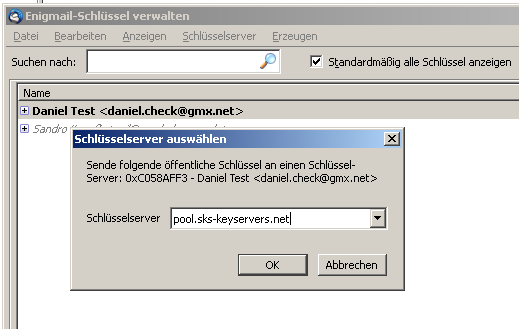
\includegraphics[width=0.8\columnwidth]{bilder/schluesselserver}
  }
\end{frame}

\begin{frame}
  \frametitle{\insertsection{} -- Schlüssel runterladen}
  \centering
  \only<+>{
    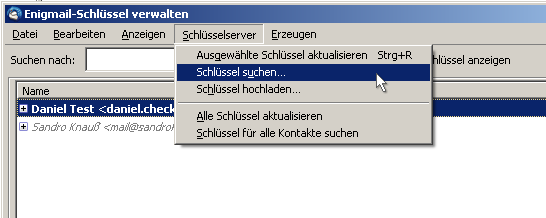
\includegraphics[width=0.8\columnwidth]{bilder/schluessel_suchen}
  }
  \only<+>{
    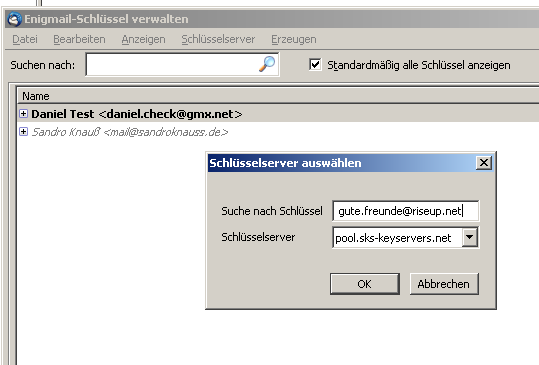
\includegraphics[width=0.8\columnwidth]{bilder/schluessel_suchen_eingabe}
  }
\end{frame}

\begin{frame}
  \frametitle{\insertsection{} -- Mail versenden}
  \centering
  \only<+>{
    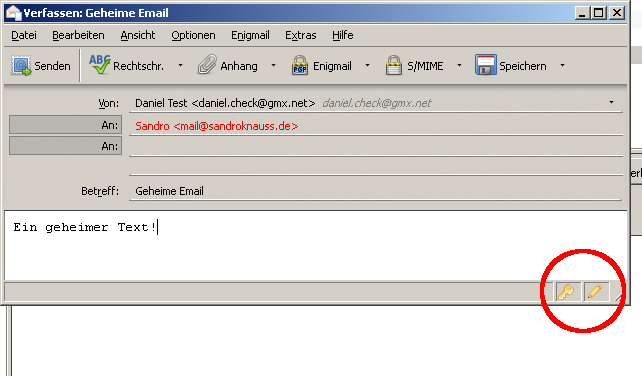
\includegraphics[width=\columnwidth]{bilder/mail_schreiben}
  }
\end{frame}

\section{Praktische Praxis}
\label{sec:praxis}

\begin{frame}
  \frametitle{\insertsection}
  \begin{itemize}
  \item GPG4Win und Enigmail runterladen
  \item Beides installieren
  \item Schlüssel erzeugen
  \item Widerrufszertifikat erzeugen und abspeichern
  \item Test-Mail schreiben
  \end{itemize}
\end{frame}

\section{Wie weiter?}
\label{sec:weiter}

\begin{frame}
  \frametitle{\insertsection}
  \begin{itemize}
  \item Skript
  \item Feedbackrunde
  \item Weitere Wünsche?
  \end{itemize}
\end{frame}

\begin{frame}
  \frametitle{War alles viel zu schwer?}
  
\includegraphics[width=1.05\columnwidth]{bilder/math4}
\end{frame}

\end{document}
